\section{Estado del arte}

\subsubsection{Exploración multi-robot}
La exploración multi-robot consiste en utilizar una flota robotica para obtener de informacion de un entorno desconocido con el proposito de generar un mapa que lo represente. 

El uso de varios robots es util porque introduce redundacia, aumentando la tolerancia a fallos. Por otro lado la exploracion suele ser altamente paralelizable ya que en un mismo instante de tiempo suelen haber varios lugares en los cuales un robot puede obtener informacion, por lo que aumentar la cantidad de recursos roboticos es esperable que se reduzcan los tiempos de exploración\cite {cao1997cooperative}\cite{dudek1996taxonomy}\cite{guzzoni1997many}. Sin embargo aumentar el numero de robots en la flota de exploracion, aumenta el riesgo de que estos se interfieran entre si, causando perdidas de tiempo en desvíos para evitar colisiones\cite{guzzoni1997many}\cite{goldberg1997interference}. Esto determina que existe un numero optimo de robots en una flota, en el cual se logra un balance entre la capacidad de explotar el paralelismo en la exploracion y el tiempo perdido por interferencias. Un mecanismo de coordinación que logre evitar interferencias suele ser un factor critico en la exploracion multirobot porque permite lograr el balance anteriormente mencionado con una cantidad de robots mayor al que se podria tener sin coordinar\cite{nieto2014coordination}.

no se bien si esta sección va como parte del estado del arte o seria parte de la intro. Algunas cosas que se pueden incluir en esta son:

  Descripción genérica del problema

  Aspectos a considerar

  Problemas relacionados

  Soluciones posibles a alto nivel

\subsection{Mapas}\cite{Liu2015}\cite{Thrun1998}
Un mapa consiste en un modelo de un entorno, en el contexto de la robótica los mapas se pueden dividir en dos categorías, \emph{mapas métricos} y \emph{mapas topológicos}.

Los mapas métricos son mapas principalmente caracterizados por representar la geometría de todo el entorno, incluyendo a su vez una escala que permite asociar las dimensiones representadas dentro del mapa con la realidad.

Los mapas topológicos por otro lado son mapas simplificados al punto de solo incluir regiones topológicas y conexiones entre estas. Normalmente se representan con grafos donde las regiones de interés son los vertices y las aristas son las conexiones entre ellas.

La simplicidad de los mapas topológicos es útil para ayudar a los humanos a entender un entorno (por esto es usual ver mapas topológicos de sistemas de transporte) y permiten instrucciones que nos resultan naturales, por ejemplo, \say{ir a la habitación A}.

Dicha simplicidad también causa que para un mismo entorno los mapas topológicos suelan ser varios ordenes de magnitud mas pequeños que los mapas métricos y por lo tanto, mas allá de la memoria que se ahorra también se tiene una planificación mas eficiente. Sin embargo la falta de detalle en la representación hace que los planes de navegación obtenidos de un mapa topológico suelan ser peores que los obtenidos en mapas métricos.

\subsubsection{Grilla de ocupación}
Una grilla de ocupación es un mapa métrico que se basa en una teselación del espacio en celdas, donde cada celda almacena una estimación probabilística de su estado (libre, ocupado, etc). 

% TODO
% En esta seccion se debe tratar:

% que es una grilla de ocupación.

% Para que sirve en general

% Se puede contruir un GVD a partir de una grilla de ocupación. (quizas despues?)

% \subsection{Representación poligonal}
% Las representaciones poligonales son mapas métricos propuestos como alternativas a las grillas de ocupación, que busca


\subsubsection{Mapas topológicos basados en regiones}
Una gran parte de los mapas topológicos se basa en segmentar el espacio en regiones de interés que serán las regiones topológicas del mapa. 

El concepto de region de interés es equivalente al de habitaciones y corredores en entornos estructurados como lo son las casas y oficinas.

\subsection{Diagrama de Voronoi}\cite{choset2005principles}\cite{Thrun1998}
Dado un espacio de trabajo $W$, $S \subset W$ es un conjunto de puntos llamados \emph{sitios}. Sea $p\in W$, la función $d_p : W \rightarrow R$ computa la distancia entre dos puntos en $W$. Una \emph{region de Voronoi}\ref{eq:regV} $R_i\subset W$ es el conjunto de puntos mas cercanos a un sitio $s_i\in S$ particular.
\begin{equation}
  R_i = \{p \in W : d_p(s_i) \leq d_p(s_j), s_i,s_j\in S,s_j \neq s_i\}\label{eq:regV}
\end{equation}
De forma similar $BP_p \in S$ \ref{eq:bases} es el conjunto de sitios mas cercanos a un punto $p \in W$ que se denominan \emph{puntos bases} de $p$.
\begin{equation}
  \mli{BP}_p =\{s_i : d_p(s_i) \leq d_p(s_j), s_i,s_j\in S,s_j \neq s_i\}\label{eq:bases}
\end{equation}
Un \emph{diagrama de Voronoi} $\mli{VD}\in W$ \ref{eq:DV} se define como todos los puntos con dos o mas sitios a una misma minima distancia, o lo que es equivalente, que tienen dos o mas puntos base.
\begin{equation}
  \mli{VD} = \{p \in W : |\mli{BP}_p| \geq 2\}\label{eq:DV}
\end{equation}

Las fronteras de las regiones de Voronoi forman parte del diagrama de Voronoi por lo que es posible decir que un diagrama de Voronoi secciona el espacio en regiones de Voronoi. En la figura \ref{fig:ejemploVoronoi} se muestra un ejemplo de un diagrama de Voronoi, con $sitios=\{A_i | 0\leq i \leq 10\}$.

Una propiedad de los diagramas de Voronoi es que los puntos que pertenecen a el serán máximos locales (no estrictos) de distancia a los sitios. Esta propiedad es útil en el contexto de la robótica porque permite asegurar que los caminos en un diagrama de Voronoi generado con el conjunto de obstáculos como sitios, son seguros en tanto mantienen la mayor distancia posible a los obstáculos.

\begin{figure}[ht]
  \center
  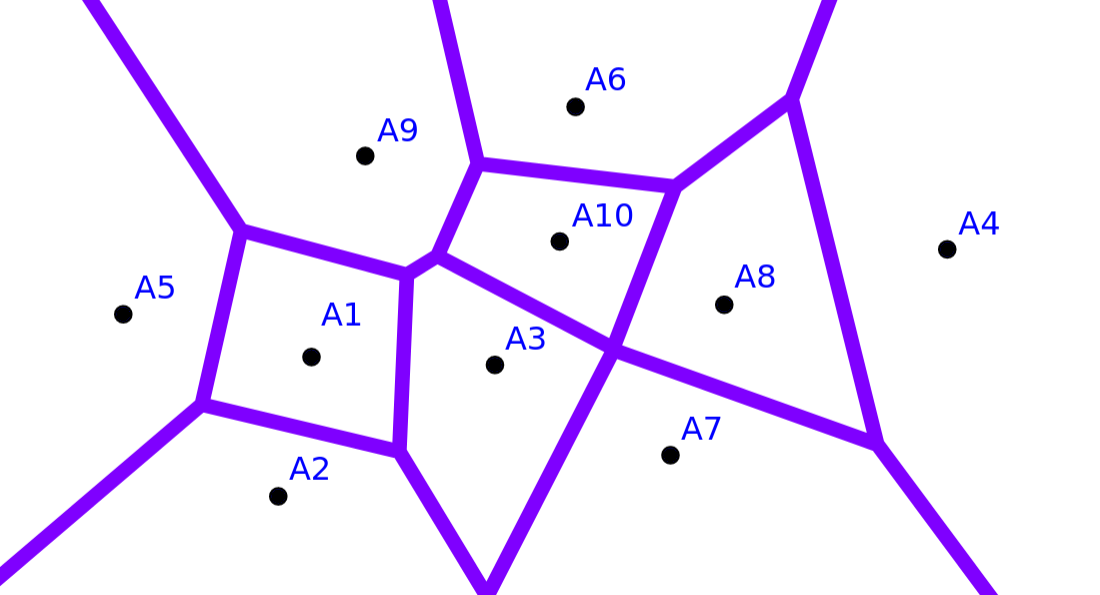
\includegraphics[width=5.5cm]{imagenes/VD.png}
  \caption{Ejemplo de un diagrama de Voronoi con diez sitios.\cite{voronoigeo}}\label{fig:ejemploVoronoi}
\end{figure} 

\subsection{Diagrama generalizado de Voronoi}\cite{choset2005principles}\cite{latombe1991}\cite{wurm2008coordinated}
Recordando que los sitios en un diagrama de Voronoi son puntos, se tiene un problema al querer utilizar obstáculos como sitios. El problema se debe a que normalmente, los obstáculos no pueden representarse como puntos en el espacio, para solucionar esto se generaliza la definición de diagrama de Voronoi para poder definirlo a partir de sitos de mayor orden, como lo son lineas, o polígonos. A esta generalización se la denomina como \emph{diagrama generalizado de Voronoi}(GVD) y los sitios de mayor orden o sitios generalizados serán representados como conjuntos de puntos del espacio de trabajo $\mli{GS}\subset 2^{W}$.

Las definiciones planteadas para los diagramas de Voronoi son similares a las utilizadas en los diagramas generalizados de Voronoi (GVD), solo es necesario cambiar la función de distancia para ser compatibles con las formas de los sitios generalizados. Para lograr esto solo es necesario intercambiar la función de distancia $d_p$ a la función de distancia generalizada $\mli{gd}_p : 2^{W} \rightarrow R$ que se define a partir de $d_p$ como se muestra en \ref{eq:dg}. Las regiones generalizadas de Voronoi $\mli{GR}_i$, los puntos base generalizados $\mli{GBP}_p$ y el diagrama generalizado de Voronoi $\mli{GVD}$ se definen según se muestra en \ref{eq:GR}, \ref{eq:GBP} y \ref{eq:GVD} respectivamente. Notar que la definición de puntos base generalizados tiene una modificación adicional al cambio en la función de distancia, esta es que en lugar de devolver los sitios generalizados mas cercanos $\mli{GBS}_p$\ref{eq:GBS}, solo devuelve los puntos mas cercanos de estos.
\begin{equation}
  \mli{gd}_p(s_i) = \min_{p'\in s_i}\{d_p(p')\} \label{eq:dg}
\end{equation}

\begin{equation}
  \mli{GR}_i = \{p \in W : \mli{dg}_p(s_i) \leq \mli{dg}_p(s_j), s_i,s_j\in S,s_j \neq s_i\}\label{eq:GR}
\end{equation}

\begin{equation}
  \mli{GBS}_p = \{s_i : \mli{dg}_p(s_i) \leq \mli{dg}_p(s_j), s_i,s_j\in S,s_j \neq s_i\}\label{eq:GBS}
\end{equation}

\begin{equation}
  \mli{GBP}_p =\bigcup_{s_i \in \mli{GBS}_p} \argmin_{p'\in s_i}\{d_p(p')\}\label{eq:GBP}
\end{equation}
\begin{equation}
  \mli{GBP}_p =\{p' : d_p(p') \leq d_p(p''), p' \in s_i, p'' \in s_j, s_i,s_j \in S,p' \neq p''\}
\end{equation}

\begin{equation}
  \mli{GVD}  = \{p \in W : |GBP_p| \geq 2\}\label{eq:GVD}
\end{equation}

% En la figura \ref{fig:ejemploGVD} se muestra un ejemplo de un GVD, el espacio libre se marca con blanco, el ocupado con negro y el GVD con azul. 
% \begin{figure}[ht]
%   \center
%   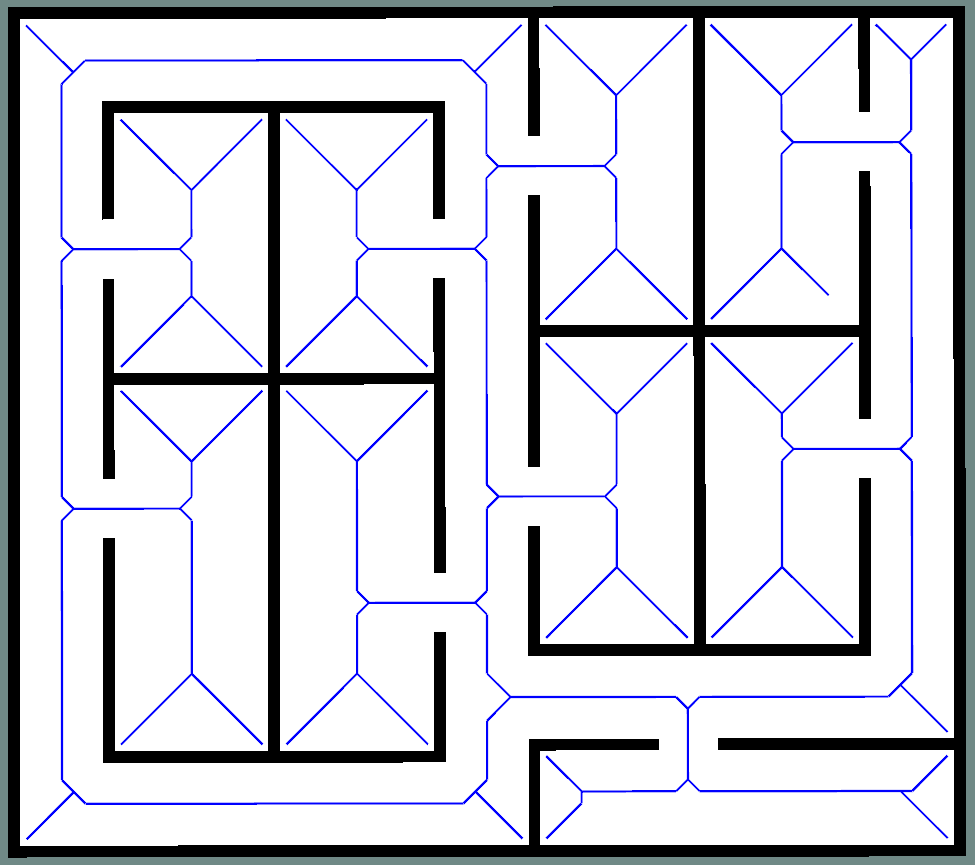
\includegraphics[width=5.5cm]{imagenes/GVD.png}
%   \caption{Ejemplo de un diagrama generalizado de Voronoi.}\label{fig:ejemploGVD}
% \end{figure} 

Es posible representar un GVD con un grafo en el cual los vertices son los puntos pertenecientes al GVD, y existen aristas entre dos vertices si estos son adyacentes en el espacio. Por otro lado otra forma mas compacta es que los vertices sean los puntos $p$ del espacio tal que $|\mli{GBP}_p|\geq 3$ y que haya aristas entre los vertices que puedan alcanzarse por caminos formados por puntos adyacentes pertenecientes al GVD. Para referirse a la segunda forma, mas compacta, de representar el GVD con un grafo se utilizara el termino grafo colapsado, y para la primera forma, el termino utilizado es grafo descolapsado.

\subsection{Mapa vial}\cite{choset2005principles}
Un mapa vial (del ingles roadmap) es un concepto normalmente representado con grafos, cuyos vertices son puntos no obstaculizados, es decir, del espacio libre $W_{libre} \subset W$ y sus aristas implican la existencia de caminos disjuntos entre los vertices. La idea principal es que un mapa vial captura la topología del espacio según el cual fueron creados y los robots lo utilizan para navegar, es decir que a partir de un mapa vial se puede planificar un camino entre dos puntos cualquiera del espacio libre 

Por lo tanto un mapa vial $\mli{MV}$ se define como un grafo que cumple con 3 propiedades fundamentales para asegurar la navegación es posible a partir del mapa vial, las propiedades son:

\begin{enumerate}
\item Accesibilidad: Para todo $p_{inicio} \in W_{libre}$ existe un camino a un $p'_{inicio}$ Nodo de $MV$.
\item Conectividad: Existe un camino entre cualquier par vertices de $\mli{MV}$ $p'_{inicio}$ y $p'_{fin}$.
\item Capacidad de salida: Para todo $p'_{fin}$ nodo de $\mli{MV}$ existe un camino a un $p_{fin} \in W_{libre}$.
\end{enumerate}

Estas propiedades aseguran la navegación, porque que dados dos puntos $p_{inicio},p_{fin}\in W_{libre}$ es posible construir un camino entre ellos. Primero por \emph{accesibilidad} se tiene un camino entre $p_{inicio}$ y un $p'_{inicio}$ Nodo de $\mli{MV}$, luego por \emph{capacidad de salida} se asegura la existencia de un  $p'_{fin}$ nodo de $\mli{MV}$ desde el cual hay un camino a $p_{fin}$ y finalmente por \emph{conectividad} se sabe que existe un camino entre $p'_{inicio}$ y $p'_{fin}$. Entonces uniendo los caminos $p_{inicio} - p'_{inicio}$(por accesibilidad), $p'_{inicio} - p'_{fin}$(por conectividad) y $p'_{fin} - p_{fin}$(por capacidad de salida) se tiene un camino que conecta dos puntos genéricos del espacio libre $p_{inicio}$ y $p_{fin}$.

En \cite{choset2005principles} se demuestra que los GVD que utilizan obstáculos como sus sitios cumplen con las 3 propiedades necesarias para ser mapas viales, lo cual justifica su uso para la navegación.




\subsection{Construcción de un GVD} 
TODO
En esta seccion dar un algormo para esto simple y no incremtal, basicamente sacarlo wurm y nuestra solucion de TSCF.
despues de grillas de ocupacion porque las usa

\subsection{Mapa topológico a partir de un GVD}
En \cite{Thrun1998} Thrun propone un método de segmentación del espacio a partir de mapa representado con una grilla de ocupación.. La idea principal del algoritmo de segmentación presentado es que las entradas y salidas entre los segmentos son pasajes estrechos, y por lo tanto encontrar estos pasajes estrechos permite delimitar segmentos. En este caso el objetivo de segmentar el espacio en habitaciones y corredores, es el de generar un mapa topológico en el cual los segmentos serán las regiones de interés.

Para describir el método de segmentación necesario introducir tres nuevos conceptos asociados al GVD, el primero es el concepto de despeje (del ingles clearance) $D : W \rightarrow R$ de un punto $p$, que equivale a la distancia entre $p$ y alguno de sus puntos base generalizados $\mli{GBP}_p$ (recordar que todos están a una misma minima distancia). El segundo es el de los puntos criticos $C\in W_{libre}$ de un GVD, un punto cumple con ser critico si pertenece al GVD y es un mínimo local según el despeje \ref{eq:crit}. El tercer y ultimo concepto es el de linea critica, que son las lineas que conectan a un punto critico $p \in C$ con sus puntos base $\mli{GBP}_p$.

\begin{equation}
  p\ \in C \iff p \in \mli{GVD},\ D(p) < D(p')\ \forall p' \in \mli{GVD} \ adyacente\_a\ p \label{eq:crit}
\end{equation}

El algoritmo comienza por la construcción del GVD, posteriormente se encuentran los puntos críticos asociados a dicho GVD para luego obtener las lineas criticas para cada punto critico encontrado. Finalmente los segmentos serán las regiones delimitadas por las lineas criticas.

La idea subyacente de este algoritmo es que, por definición, los puntos críticos se encuentran presentes en el centro de todo pasaje estrecho siendo sus puntos base los extremos de dicho pasaje. Por lo tanto las lineas criticas estarán ubicadas a lo largo de cada pasaje estrecho y dada la consideración que las transiciones entre los segmentos se dan en los pasajes estrechos, las lineas criticas actúan naturalmente como limites entre cada segmento.

TODO describir bien el algoritmo no incremental de Liu ming

\subsection{Forma alternativa de generar mapas topologicos}
Incluir el articulo que habla de la generacion de mapas topologicos con el contorno 

\subsection{Criterios de calidad de un mapa topológico}
Según \cite{Liu2015} un mapa topológico basado en regiones se considera útil si representa la estructura del entorno de manera correcta y eficiente. Para ello, consideran dos criterios, la calidad asociada a cada region y la topología la segmentación. Los criterios propuestos se basan principalmente en intuiciones geométricas. 

\subsubsection{Calidad de una region}
Los autores determinan que existen dos aspectos que intervienen en la calidad de una region, la convexidad $c_i$ y la compacidad $s_i$, específicamente, definiendo la calidad de una region como $q_i = c_i - s_i$. Adicionalmente se menciona que tanto $c_i$ como $s_i$ pueden ser multiplicados por pesos en el calculo de $q_i$ para  para hacer énfasis en una u otra característica.

\paragraph{Convexidad}
Esta se puede representar como el cociente entre el area de la region y el area de su envolvente convexa. La envolvente convexa de una region se define como el polígono convexo de menor area que contiene a la region. Un polígono convexo cumple que para cualquier par de puntos que pertenecen a la frontera del polígono, el segmento de recta que los conecta estará contenido en dicho polígono. Entonces sea $A_i$ el area de la region $R_i$ y $H_i$ el area de su envolvente convexa, la convexidad para esta region sera:
\begin{equation}
  c_i=\frac{A_i}{H_i}
\end{equation}
Se cumple que $A_i \leq H_i$ siendo iguales cuando la region es convexa, por lo tanto $c_i$ sera igual a uno cuando la region es convexa, y su valor disminuirá entre más difiera el area de la region con la de su componente convexa. En la figura \ref{fig:ejemplConvexidad} se muestra a modo de ejemplo el valor de convexidad $c$ asociado a dos regiones con distinta convexidad.
\begin{figure}[ht]
  \center
  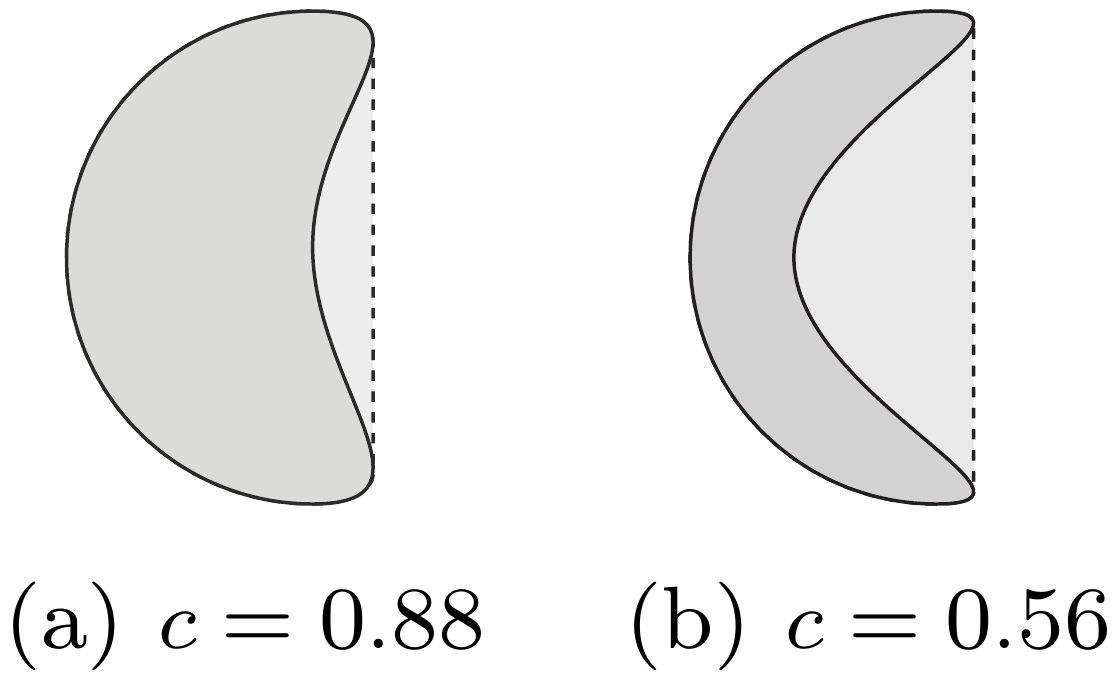
\includegraphics[width=5.5cm]{imagenes/convexidad.png}
  \caption{Dos regiones con su valor de convexidad asociado, las lineas solidas delimitan la region y las lineas punteadas delimitan su envolvente convexa. Extraído de \cite{Liu2015}.}\label{fig:ejemplConvexidad}
\end{figure} 

\paragraph{Compacidad}
% Cuanto mas cercanos son los puntos que componen una region a su centro mas compacta sera la region.
La compacidad de una region mide la distribución una region con respecto a su centro de masa. La compacidad $s_i$ de una region $R_i$ se calcula a partir de una discretization de dicha region en celdas de dimensiones y peso uniforme, llamadas elementos de masa. La ecuación \ref{ec:compacidad} define la compacidad $s_i$ para un region $R_i$, donde $x_j$ e $y_j$ son las coordenadas x e y de los elementos de masa de $R_i$, $M_i$ es igual a la cantidad de dichos elementos de masa y $x_0$ e $y_0$ son las coordenadas del centro de gravedad de $R_i$.
\begin{equation}
  s_i=\frac{1}{M_iA_i}\sum_j \frac{(x_j-x_0)^2 + (y_j-y_0)^2}{A_i} \label{ec:compacidad}
\end{equation}
Notar que cuanto mas compacta sea una region menor sera su valor $s_i$ (si se entiende por region compacta una region en la cual sus puntos interiores son cercanos al centro de masa).

\subsubsection{Calidad de segmentación}
Para determinar la calidad general de la segmentación, sera necesaria, ademas de la calidad de cada region, la calidad de las características globales de la segmentación. Para lograr determinar dichas características se definen varios indicadores que se mencionarán a continuación.

\paragraph{Cobertura}
En el caso ideal cada punto del entorno esta asociado a una region en el mapa topológico, pero por diversas razones este puede no ser el caso. Dado esto se define la cobertura $C$ de una segmentación como el cociente del area representada por el mapa topológico y el area del mapa:
\begin{equation}
C=\frac{\sum^N_{i=1} A_i}{A_m}
\end{equation}
Donde $A_m$ es el area total del mapa y $N$ es el numero de regiones.

\paragraph{Validez}
La validez $V$ de una segmentación se define como el cociente entre el numero de regiones validas y el numero total de todas las regiones:
\begin{equation}
  V=\frac{\#regiones\ validas}{\#total\ de\ regiones}
\end{equation}
Se considera que una region valida debe ser accesible por los robots utilizados. Teniendo esto en cuenta una region será valida si cubre un area mayor a $A_{min}$ y tiene al menos una entrada de ancho mínimo $l_{min}$, siendo los valores $l_{min}$ y $A_{min}$ definidos a partir las dimensiones de los robots utilizados.

\paragraph{Simplicidad}
Dado que una de las ventajas principales de los mapas topológicos es su simplicidad, que permite ayudar a una navegación y planificación eficiente, los autores consideran que es de utilidad penalizar a los mapas topológicos que tengan una cantidad elevada de regiones, considerando dicha cantidad como un indicador de complejidad. 

La simplicidad $S$ de una segmentación se define en la ecuación \ref{ec:simp} donde $\hat{N}$ es el numero esperado de regiones y $\phi$ refleja el impacto que tiene la diferencia entre el numero de regiones esperado y el obtenido. $\hat{N}$ y $\phi$ son parámetros a definir dependiendo de la aplicación.

\begin{equation}
  S=e^{-\frac{|N-\hat{N}|}{\phi}} \label{ec:simp}
\end{equation}


\subsubsection{Calidad general}
Finalmente, evaluar la calidad general $Q$ de una segmentación, se reduce a combinar la calidad cada región y los indicadores de calidad de la segmentación, según la siguiente ecuación:
\begin{equation}
Q=\frac{CV}{N}\sum^N_{i=1}{q_i+\lambda S}
\end{equation}

Donde $\lambda$ es un peso que determinara la importancia de la simplicidad de la segmentación en cálculo calidad general de la segmentación.

\subsection{Eficiencia en la construccion de GVD y mapa topologicos a partir de GVD}
en esta seccion se trataria sobre las diferencias entre incremental y no incremental, mencionar lo que se gana en performance y que implica una dificultad mayor, y despues comentar bien como es la:

generacion de GVD incrmental

segmentacion incremental (mencionar tambien que la contorno tambien tiene variante incrmental)

Luego comentar nueveametne las tecnicas de remoción de falsos positivos de Wurm y la diferencia entre utilzarlas y no (usar de ejemplo resultados de Liu ming) esto para decir que una de las cosas que se hace en el desarrollo es generar un algoritmo que hace esto


\subsection{Coordinación a partir de mapas topológicos}
Incluir aca a wurm la parte de coordinacion

\subsection{Coordinación a partir de la segmentaciones alternativas del entorno}
Hablar aca de otras forma de coordinar a partri de la segmentacion que no sean mapas topologicos:

El que segmenta a partir de los centros de los robots

El que segmenta haciendo k-means de las zonas desconocidas

\subsection{No se bien como nombrar esto}
Se puede incluir cosas mas genericas de la exploracion multirobot, esto puede incluir la solucion de guillermo y su criterio de parada anticipado. Y tambien podria incluir las soluciones propuestas en el paper que describe paquetes de exploracion, que entre otras cosas permite mencionar el paquete ad-hoc y el problema de las comunicaciones no perfetas que esto intenta solucionar.

\subsection[Coordinated Multi-Robot Exploration using a Segmentation of the Environment]{Coordinated Multi-Robot Exploration using a\\ Segmentation of the Environment}

\cite{wurm2008coordinated}
El articulo describe y analiza un enfoque de coordinación para la exploración multi-robot que se basa en la distribución eficiente de los robots al explorar el entorno, teniendo en cuenta la estructura de dicho entorno. Para lograr la distribución el entorno se divide en segmentos, por ejemplo, correspondientes a habitaciones y corredores. Luego, las asignaciones de robots a objetivos se hacen considerando que los robots deben ser distribuidos de forma uniforme sobre los segmentos identificados. 

% Y en lugar de considerar todas las fronteras entre áreas desconocidas y exploradas como ubicaciones objetivo, se envían los robots a los segmentos individuales con la tarea de explorar el área correspondiente.
En el articulo se describen dos tareas principales: la segmentación del mapa y la asignación de objetivos a los robots.

\subsubsection{Segmentación del mapa}
% La segmentación de mapas se basada en la partición de un grafo.  
% , como lo son los grafos de Voronoi
En el articulo el mapa es representado como un grafo de Voronoi, para calcular el grafo de Voronoi $G(m) = (V, E)$ asociado a un mapa $m$, se considera el conjunto $O_p (m)$ que contiene para cada punto $p$ en el espacio libre $C$ de $m$ el conjunto de puntos de obstáculos más cercanos. El conjunto $V$ de nodos del grafo de Voronoi es definido como el conjunto de puntos $p$ en $C$ para los cuales hay al menos dos puntos de obstáculo a distancia mínima, existiendo una arista entre dos nodos si sus puntos correspondientes en $m$ son adyacentes:
\[
V = \{p \in C : |O_p (m)| \geq 2\}
\]
\[
E = \{(p, q) : p, q \in V, p \text{ adjacent } q \text{ in } m\}
\]

El grafo de Voronoi se puede generar a partir de una grilla de ocupación, aplicándole la transformación de distancia euclidiana\cite{meijster2002general} se obtiene como resultado un mapa de distancia que mantiene para cada celda de la grilla la distancia al obstáculo más cercano, a partir del cual es posible determinar $V$ y $E$ como se describió anteriormente.
% (o de interés para explorar, normalmente corredores o puertas)
%, los cuales normalmente se ubican en puertas 

La segmentación de mapas se basa en la partición del grafo utilizado para representar el mapa, y se realiza a partir de los denominados puntos críticos, definidos como puntos que cumplen con ser mínimos locales según la distancia a los obstáculos. La idea es utilizar los puntos críticos para reconocer pasajes entre dos habitaciones o entre habitaciones y corredores. Dado que la forma de los pasajes suelen generar puntos críticos en ellos, el problema pasa a ser el de evitar reconocer falsos positivos (puntos críticos que no estén en un pasaje). Con el motivo de evitar falsos positivos los puntos críticos se restringen a los nodos del grafo que sean mínimos locales según la distancia a los obstáculos, de grado 2 (tengan dos aristas), que tengan un vecino de grado 3 (un nodo de intersección entre varios caminos) y que conduzcan a áreas desconocidas.
Finalmente los pasajes reconocidos determinan una partición del grafo que a su vez determina los segmentos, que por estar entre pasajes serán corredores y habitaciones.

\subsubsection{Asignación de objetivos}
% Los entornos interiores son en general estructurados, por ejemplo, los edificios generalmente se dividen en habitaciones a las que se puede llegar por pasillos.
Los objetivos serán, como es usual, las fronteras entre las partes desconocidas y conocidas del mapa.

Asignar más de un robot a un mismo segmento en muchos casos, puede ser una desventaja, ya que el segmento podría ser demasiado pequeño para que un segundo robot acelere su exploración, aunque inicialmente haya más de una frontera en el mismo o, por otro lado, al terminar la exploración de un segmento, los robots pueden incluso bloquearse entre sí mientras intentan abandonarlo, lo que aumentará el tiempo de exploración. Por lo tanto, el objetivo es distribuir uniformemente a los robots sobre los segmentos.

Para resolver la asignación se propone utilizar el método húngaro, a partir de los costos $C_{s}^{i}$ definidos como el costo de llegar a la celda frontera más cercana del segmento $s$ con el robot $i$, descontando un valor constante en caso de que el robot ya se encuentre en el segmento. El método húngaro da soluciones que evitan tener más de un robot por segmento mientras esto sea posible, y asigna más de un robot a un segmento en el caso de que haya más robots que segmentos. Esta descripción corresponde al algoritmo \ref{alg:asignacionobjetivos}.

\begin{algorithm}
\SetAlgoLined
    Determinar segmentos $S = \{s_{1} , ..., s_{n} \}$ del mapa\\
    Determinar el conjunto de fronteras objetivo para cada segmento\\
    \For{cada robot $i$}{
        \For{cada segmento $s \in S$}{
                Computar el costo $C_{s}^{i}$\\
                Descontar al costo $C_{s}^{i}$ si el robot $i$ ya se encontraba en $s$\\
            }
    }
    Asignar robots a los segmentos usando el método húngaro\\
    \For{cada segmento $s \in S$}{
        Asignar robots a las fronteras objetivas en $s$ utilizando el método húngaro\\
    }
    \caption{Asignación de objetivos}
    \label{alg:asignacionobjetivos}
    
\end{algorithm}

Usando este enfoque, cada uno de los corredores es explorado completamente por uno de los robots revelando rápidamente la estructura de un edificio, mientras que se asignarán otros robots a las habitaciones accesibles desde los corredores a medida que estas se vayan detectando.



% \section{Investigación previa}
% Con el motivo de introducirnos y orientar el trabajo, se investigaron cuatro artículos relacionados al problema de la exploración multi-robot. A continuación se describirá cada uno de los artículos, haciendo especial énfasis en las características de los mismos que se relacionan con el trabajo realizado.
\subsection{A novel stop criterion to support efficient Multi-robot mapping}\cite{amorin2019novel}
El articulo modela e implementa una solución al el problema de coordinación y exploración de un entorno desconocido a partir de un sistema de robots homogéneos, con el objetivo de analizar un criterio de terminación novedoso basado en la ganancia de información esperada.

% El articulo consta de varias secciones: la representación del entorno, los componentes(robot y estación central) y comunicaciones entre ellos, método de identificación de tareas para cada robot y el criterio de finalización.

\subsubsection{Representación del entorno}
El entorno $E$ se define como un espacio de trabajo plano limitado limitado $E\subseteq R^2$. Para que sea computacionalmente tratable dicho entorno $E$ está representado por una estructura de grilla de ocupación donde cada celda $c$ puede pertenecer a tres estados probabilísticos diferentes $S = \{f, o, u\}$, representando libre, ocupado y desconocido, respectivamente. Para realizar las asignaciones solo se considerara el centro de la celda.

\subsubsection{Componentes y comunicaciones}
La flota se compone de $N$ robots móviles circulares rígidos con capacidad para tomar mediciones en toda la circunferencia alrededor con un radio $r$. Existe una estación central encargada de la tarea de reconocimiento de objetivos y asignación de los mismos. Los robots serán quienes recopilen la información del entorno y la central la encargada de crear un mapa global a partir de esta. 

En el articulo, se consideran comunicaciones ideales, suponiendo que los robots no tienen restricciones de comunicación (por ejemplo, sin errores ni pérdidas con ancho de banda y alcance ilimitados). %Cabe aclarar que las comunicaciones inalámbricas son importantes en el contexto de exploración multi-robot.

\subsubsection{Método de identificación y asignación de tareas}

Las celdas que llevan a espacios desconocidos, consideradas como libres y que son adyacentes a celdas desconocidas, son denominadas celdas frontera (fronteras), en tanto conforman una frontera entre espacios libres y desconocidos. Las fronteras son objetivos potenciales de exploración ya que si el robot alcanzara dicha celda este podría recopilar nueva información dentro del radio de sensado. Sin embargo, el tratamiento de todas las fronteras como tareas de exploración diferentes podría ser computacionalmente prohibitivo. Por lo tanto, para reducir la carga, se intenta determinar las celdas frontera mas significativas, para lograr esto se hace lo siguiente, primero, las fronteras se dividen en conjuntos disjuntos $F_k$. 
Luego, se obtienen las fronteras mas significativas de cada conjunto $F_k$ considerando el radio de sensado de un robot de forma que si dos robots van a dos celdas frontera significativas distintas de $F_k$, sus radios de sensado no se solapen, esto se hace utilizando el algoritmo K-Means. Finalmente las fronteras consideradas significativas para algún $F_k$ se convierten en celdas objetivo, también conocidas como tareas de exploración.

La asignación de tareas se resuelve organizando una subasta entre robots. Cuando un robot completa una tarea (llegando a una celda objetivo), este envía una notificación a la estación central. La Estación Central comparte la última versión del mapa con la flota e inicia un proceso de subasta solicitando postores. Durante un corto período de tiempo, cada robot no asignado es notificado, pudiendo enviar una oferta; cada oferta consiste en una lista de pares tarea-utilidad, donde la utilidad considera tanto la estimación de ganancia de información como el costo asociado a la ruta necesaria para cumplir con la tarea. Finalmente la central, a partir de las listas de todos los postores, resuelve las asignaciones de forma voraz, para luego notificar a cada robot su tarea asignada.
% Dada la falta de conocimiento sobre el entorno, la mejor opción para los robots es visitar los lugares donde la ganancia de información puede ser potencialmente mayor, sin dejar de considerar el esfuerzo necesario llegar al objetivo, por lo tanto, los robots priorizarán las tareas por el coeficiente entre la ganancia de información esperada y el esfuerzo esperado necesario para completar la tarea.

El valor de la ganancia de información de cada frontera resultante debe ser estimado, en el artículo se presenta un estimador de ganancia, el cual se basa en el rango de visión del robot y el entorno conocido. 

\subsubsection{Criterio de parada}

El criterio según el cual detener la exploración es un aspecto importante de la exploración multi-robot. Una de las opciones sería la configuración del sistema para que, al llegar a un porcentaje de cubrimiento del entorno, la exploración sea detenida. Esta medida en la práctica no es efectiva, solo sirve en caso de tener conocimiento del mapa global. Otra opción es que el sistema verifique de forma autónoma si existen espacios accesibles desde donde cualquier robot pueda recopilar nueva información, y detener la exploración de lo contrario.

El criterio de parada propuesto en el articulo, se basa en que durante la exploración, los robots obtienen conocimiento sobre el entorno que mejora continuamente sus habilidades de predicción. Teniendo en cuenta que una suposición básica es que la flota explora entornos limitados, las hipótesis son dos, la primera es que existe un momento a partir del cual la estimación de la ganancia de información se puede hacer con precisión (es decir, el error cometido por el estimador tiende a cero). Y la segunda es que dicho momento puede determinarse en línea mediante robots que calculan su propio error en sus estimaciones de ganancia de información. Dicho esto el criterio de parada es que dada una cierta tolerancia cada robot da por concluida su participación en la exploración cuando para $n$ objetivos seguidos, dicha tolerancia es mayor a la diferencia entre la estimación de ganancia de información que se hizo para un objetivo y la ganancia de información real. La idea subyacente es que tan pronto como los robots obtengan suficiente información sobre el entorno como para poder estimar la porción inexplorada con precisión, estos podrán detenerse.

\subsection[Voronoi-Based Space Partitioning for Coordinated Multi-Robot Exploration]{Voronoi-Based Space Partitioning for Coordinated\\ Multi-Robot Exploration} \cite{wu2007voronoi}

% Este artículo describe y evalúa la extensión de un algoritmo de exploración multi-robot y muestra que al reemplazar el modelo de mapa original (una grilla de ocupación) con una representación poligonal más compacta y flexible, el nuevo enfoque aumenta significativamente la eficiencia de la etapa más costosa del algoritmo original, que es la división de áreas desconocidas en tantas regiones como robots. El algoritmo de agrupación K-Means original se sustituye por un algoritmo de partición basado en Voronoi aplicado a polígonos.
Las grillas de ocupación es una de las representaciones de mapas mas utilizadas en el contexto de exploración multi-robot, sin embargo, estas grillas no son apropiadas para entornos que son muy grandes o cuyos límites no están bien delimitados desde el comienzo de la exploración. En contraste, las representaciones poligonales no tienen tales limitaciones.

El artículo propone utilizar una representación poligonal en la cual el mapa consiste en la union de conjunto de polígonos cerrados de forma y tamaño arbitrario, que pueden estar libres, no explorados u obstaculizados. 

El desempeño de la representación propuesta se comprueba contra una estrategia de exploración multi-robot que hace uso de grillas de ocupación, de lo cual se concluye que una representación poligonal es más compacta, flexible y logra aumentar significativamente la eficiencia.

\subsubsection{Representación poligonal}
Inicialmente, todo el mapa estará constituido por un solo polígono desconocido. A partir de lo sensado por cada robot, se incluye nueva información sobre entorno a la representación agregando polígonos libres y ocupados que son substraídos de los polígonos desconocidos a los que pertenecían.

Los objetivos de exploración se determinan a partir de las aristas entre polígonos desconocidos y polígonos libres denominadas como aristas frontera que son análogas a las celdas frontera de las grillas de ocupación.

El trabajo propone asignar tareas a partir de la division el entorno desconocido en tantas regiones como robots existan en la flota, para luego asignar a cada robot la tarea de explorar una region diferente. El entorno se divide a partir de un algoritmo que adapta al algoritmo K-Means para funcionar a partir de la representación poligonal propuesta, este algoritmo se explica en la sección\ref{subsubsec:particionamientovoronoi}.

%La division del entorno se logra adaptando el algoritmo K-means para funcionar en utilizado para encontrar los centroides correspondientes a las agrupaciones de áreas desconocidas, ya que se asume que estos serán los puntos más provechosos para que los robots exploren.

Finalmente, la planificación del camino del robot es realizada en el interior de los polígonos libres, cosa que se puede hacer a partir de la aplicación de cualquier algoritmo de descomposición celular, por ejemplo el que se explica en \cite{schachter1978decomposition}.
   
\subsubsection{Particionamiento basado en polígonos}\label{subsubsec:particionamientovoronoi}
El diagrama de Voronoi\cite{fortune1987sweepline} de un conjunto de puntos 2D, también conocidos como sitios, $C_{i} , 1 \leq i \leq K$, es una partición de ese espacio en $K$ regiones convexas disjuntas conocidas como células Voronoi. Cada región $V_i$ está definida por los puntos en el espacio que están más cerca de $C_{i}$ que a cualquier otro $C_{j}$, $j\neq i$. 

Sea $n$ numero de robots, el resultado deseado es obtener un conjunto de $K=n$ celdas de Voronoi para las cuales, sus centroides (centros de masa) y sus sitios estén a una distancia menos que cierta tolerancia $\varepsilon$. % cerradas que están globalmente delimitadas por el polígono a dividir

La generación de estas celdas se realiza a partir del algoritmo \ref{alg:particionamientovoronoi} que adapta K-Means (algoritmo que encuentra clusters en un mapa discretizado) a partir de diagramas de Voronoi.

Notar que el algoritmo trabaja con celdas de Voronoi restringidas, estas son las celdas resultantes de un diagrama de Voronoi restringidas a los limites del mapa conocidos por hipótesis.

\begin{algorithm}
\SetAlgoLined
    Elegir aleatoriamente $K$ puntos $C_i$, $1 \leq i \leq K$, contenidos en los polígonos correspondientes a las regiones desconocidas actuales en el mapa.\\
    Calcular el diagrama de Voronoi asociado con el conjunto actual de $C_i$.\\
    Restringir las celdas del diagrama de Voronoi a los polígonos desconocidos actuales.\\
    Determinar el centro de masa $M_i$ de cada celda Voronoi restringida.\\
    \eIf{$C_i - M_i < \varepsilon\ \forall i$}{
        Saltar al paso 11.\\
    }{
        Sustituir cada $C_i$ por su $M_i$ correspondiente.\\ Volver al paso 2.\\
    }
    
    Dividir el conjunto de polígonos desconocidos en $K$ regiones disjuntas según las celdas de Voronoi restringidas encontradas.\\
    \caption{Particionamiento basado en Voronoi}
    \label{alg:particionamientovoronoi}
    
\end{algorithm}

%%%%%%%
% Desde acá modulo taller (redactado)
%%%%%%%
% hasta acá redactado

\subsection{Incremental reconstruction of generalized Voronoi diagrams on grids}

El principal problema con este acercamiento es que el GVD se construye basa en determinar obstáculos independientes para luego calcular el GVD. Esto es un problema porque no es claro en como pasar de celdas obstaculizadas a obstáculos que están compuestos por estas (buscar mas problemas, ineficiencia?, nuestro código no lo soportaba de antes).  El siguiente artículo propone una solución que evita esta necesidad y solo basta con tener un grilla de ocupación.

\subsection{Efficient grid-based spatial representations for robot navigation in dynamic environments}
Articulo del cual obtuvimos varias las características de nuestra implementación incremental


%%%%%%%
% Desde acá proyecto de grado redactado
%%%%%%%

\subsection[Distributed Multi-robot Exploration Based on Scene Partitioning and Frontier Selection]{Distributed Multi-robot Exploration Based on\\ Scene Partitioning and Frontier Selection}
% Al considerase una solución para el problema de exploración hay dos aspectos centrales a resolver, identificar posibles objetivos de exploración y como priorizar estos objetivos de forma de priorizar los mas relevantes.

Este articulo propone una solución distribuida al problema de exploración multi-robot%, que al igual que otras ya comentadas partición el entorno aunque en este caso dicha 

\subsubsection{Formulación del problema}
La variante del problema de exploración multi-robot tratada en este articulo es la de explorar un entorno desconocido $W\in R^2$ utilizando un conjunto de robots $R={R_1,R_2,...,R_n}$. Se utilizan celdas de ocupación, por lo que el entorno se descompone en un conjunto de celdas $C={c_1,c_2,...,c_n}$. Cada robot $R_i$ tiene:
\begin{enumerate}
  \item Un mapa $M_i \in CxL$ donde $L$ son las diferentes estados en los que puede estar una celda. 
  \item Una posición inicial $q_{init}^{i}\in R^2 \times [-\pi,\pi]$. 
  \item Un sensor $S_i$ para explorar el entorno desconocido.
\end{enumerate}

Adicionalmente asumen que existe siempre un cuadro delimitador de $W$ que puede ser establecido, aunque sea de forma aproximada, antes de que la exploración comience, comunicación perfecta (sin perdida de rango infinito) y que cada robot tiene acceso a su posición respecto a un marco de referencia común.

\subsubsection{Descripción del sistema}
El sistema tiene un diseño modular, este consta de 4 módulos que se encuentran en cada robot, el modulo de distribución de información, el modulo de asignación de zonas, el modulo de adquisición de información y el modulo de exploración. Estos se describen en las siguientes secciones. 

\paragraph{Modulo de distribución de información}
Este modulo se encarga de distribuir a los demás robots la posición del robot al que pretence, las ubicaciones que conoce de los demás robots y su mapa $M_i$. 

\paragraph{Modulo de asignación de zonas }
El entorno es segmentado en zonas y la exploración cada una de estas es asignada a un robot. El modulo de asignación de zonas es el responsable de realizar la segmentación en zonas y su posterior asignación a los robots. La segmentación genera tantas zonas $E_i$ como robots $R_i$ que $E_i$ se define en la ecuación \ref{ec:zones} a partir de la posición $C_i$ de $R_i$. .
\begin{equation}\label{ec:zones}
  E_i=\{c_j:d_g(C_i,c_j)\leq d_g(V_i(k),c_j) \forall i \neq k , c_j \in U_i\}
\end{equation}
Donde $U_i \subset M_i$ son la celdas desconocidas del mapa asociado al robot $R_i$ y $d_g(c',c'')$ es la distancia geodésica, que indica el camino compuesto de centros de celdas mas corto entre dos celdas $c'$ y $c''$ que respecta la conectividad entre las celdas que lo componen.

Cada zona $E_i$ es asignada al robot $R_i$ y este explorara las celdas de $E_i$ según lo determine el \hyperref[par:estar:moduloexp]{modulo de exploración}.

\paragraph{Modulo de adquisición de información}
El propósito de este es el de actualizar el mapa $M_i$ de el robot $R_i$ según la información obtenida por su sensor $S_i$ y su posición $C_i$.

\paragraph{Modulo de exploración}\label{par:estar:moduloexp}
El modulo de exploración esta compuesto por tres submódulos. 

El primero de ellos es el submódulo de asignación de objetivos, como su nombre lo indica, este se encarga de seleccionar un objetivo de todos los pertenecientes a la zona asignada $E_i$ para asignarlo al robot $R_i$. El objetivo seleccionado $G_i$ es el que alcanza el menor valor para la función de peso $f_p$ que se computa como \ref{ec:weight}.
\begin{equation}\label{ec:weight}
  f_p(c_j) = k_d.d_g(C_i,c_j) + k_a.\phi_i(c_j)
\end{equation}
Donde $k_d$ y $k_a$ son dos constantes positivas que determinan el peso de cada sumando, $d_g(C_i,c_j)$ hace referencia a la distancia geodésica mencionada anteriormente, $\phi_i(c_j)$ es el angulo entre la orientación del robot y el vector con origen en la posiciones del robot $C_i$, y fin en el centro de celda $c_j$. 

Luego esta el submódulo de planificación de ruta, este se encarga de generar una ruta que le permita al robot llegar al objetivo asignado. Esto se logra a partir del algoritmo $A*$, para la ejecución de este se asume que las celdas desconocidas son libres. En el caso de encontrarse un obstáculo en la ruta planificada se replanifica ejecutando nuevamente el algoritmo $A*$ en la version mas reciente del mapa.

El ultimo es el submódulo de ejecución de trayectoria que se encarga de generar los comandos de actuación para seguir una ruta planeada.

\subsection[Incremental Topological Segmentation for Semi-structured Environments using discretized GVG]{Incremental Topological Segmentation for Semi-\\structured Environments using discretized GVG}

Este articulo se centra en la descripción de un método de segmentación incremental del entorno que se basa en la propuesta por Thrun \cite{Thrun1998}. Para lograr la incrementalidad se desarrollaron variantes incrementales para la generación del GVD y para la detección de segmentos.

El algoritmo de generación incremental del GVD se basa en el desarrollado en \cite{kalra2009incremental}. 

La detección incremental de puntos críticos se hace solo considerando la definición básica de Thrun, sin considerar las técnicas de remoción de falsos positivos propuestas por Wurm \cite{wurm2008coordinated}, esto facilita la tarea de detección pero impacta negativamente los resultados. Para lograr la mencionada detección incremental de puntos críticos, se recalculan los mínimos locales según los cambios del GVD (nuevos nodos, nodos removidos, cambios de despeje) de cada incremento, específicamente se recalcula en los cambios y sus vecinos de primer y segundo grado. Al detectar nuevo punto critico se calcula la linea critica asociada.

Finalmente es necesario, a partir de las lineas criticas, determinar de forma incremental a que segmento pertenece cada celda. Para esto, se elije una celda de todas las celdas afectadas en el incremento y se la agrega a una nueva region, sus celdas vecinas que estén dentro del mapa, no estén ocupadas y no sean cruzadas por una linea critica serán agregada...



% \begin{algorithm}
% \SetAlgoLined
%     Determinar segmentos $S = \{s_{1} , ..., s_{n} \}$ del mapa\\
%     Determinar el conjunto de fronteras objetivo para cada segmento\\
%     \For{cada robot $i$}{
%         \For{cada segmento $s \in S$}{
%                 Computar el costo $C_{s}^{i}$\\
%                 Descontar al costo $C_{s}^{i}$ si el robot $i$ ya se encontraba en $s$\\
%             }
%     }
%     Asignar robots a los segmentos usando el método húngaro\\
%     \For{cada segmento $s \in S$}{
%         Asignar robots a las fronteras objetivas en $s$ utilizando el método húngaro\\
%     }
%     \caption{Asignación de objetivos}
%     \label{alg:asignacionobjetivos}
    
% \end{algorithm}


% hasta acá redactado


\subsection[Incremental contour-based topological segmentation for robot exploration]{Incremental contour-based topological\\ segmentation for robot exploration}
\subsubsection{Resumen}
Habla de mapas topológicos, estos son los mapas que se generan a partir de la segmentación del entorno. 
Específicamente se centra en describir y evaluar un algoritmo de segmentación para la contracción de mapas topológicos en 2D: Segmentación topológica basada en el contorno de los obstáculos del mapa (Contour Based Topological Segmentation).
También se describe una variante incremental para poder usarse en tiempo real para la exploración multi-robot.

\subsubsection{Notas generales}
Interesante tener en cuenta la existencia de diferentes métodos para segmentar el espacio.

Este se evalúa contra la segmentación humana.

Se describe una variante incremental para poder usarse en tiempo real para la exploración multi-robot.

En la parte de trabajos relacionados habla de la segmentación basada en GVD. <- importante

Interesante el trabajo relacionado por describir los tipos de segmentación

Funcionamiento:
\begin{enumerate}
  \item De grid 2D based map a un conjunto de polígonos:
  \begin{enumerate}
     \item De grid a imagen binaria
     \item A partir de esa imagen usando el modo árbol de la función de la biblioteca OpenCV $findCountours$ que devuelve hacer jerarquía de contornos según que contornos (padres) contienen a otros (hijos)
  \end{enumerate}
\item Luego se usa la función DuDe\_segment toma los polígonos del paso anterior para obtener la descomposición del espacio en segmentos. Esto se hace para cada polígono encontrado en 1. Y el resultado final es la union de estas segmentaciones. La descomposición DuDe se explica en: 

  \url{http://masc.cs.gmu.edu/wiki/Dude2D}
\end{enumerate}

Obtienen buenos resultados, la version incremental permite tiempo real, solo tiene un parámetro a tunear (maxima convexidad, usado en el DuDe\_segment), flexible para entornos estructurados y no estructurados. Y es independiente del tamaño de la grid, solo importan las proporciones del contorno.

\subsection[Coordinated Multi-Robot Exploration: Out of the Box Packages for ROS]{Coordinated Multi-Robot Exploration: Out of the\\ Box Packages for ROS}
\subsubsection{Resumen}
Se presentan y evalúan paquetes de ROS para la exploración multi-robot coordinada. Estos paquetes tienen el objetivo de ofrecer funcionalidades básicas para tener una solución completa pero simple para el problema de la exploración multi-robot permitiendo una configuración completamente distribuida, apuntando a que grupos de investigación puedan utilizarlos. Los paquetes son:
\begin{itemize}
  \item ad hoc communication between robots,
  \item construction of global maps from local maps
  \item exploration of unknown environments
\end{itemize}

\subsubsection{Notas}
\paragraph{WIRELESS AD HOC COMMUNICATION}

ROS permite comunicación ínter proceso local a través de un maestro usando el patron de comunicación duplicación/subscripción. El maestro se encarga de manejar los publicadores y los subscriptores a  tópicos de ROS ( canales de comunicación entre procesos ). Para hacer un sistema multi-robot en este caso seria necesario que todos los robots se conecten inalámbricamente a un solo maestro y solo este maestro es el encargado de establecer canales de comunicación entre procesos. Esto significa que dos procesos deben comunicarse con el maestro para poder luego comunicarse entre si y en el caso de desconectarse deben recaer nuevamente en el maestro para lograr una re conexión. Esto es malo ya que el maestro es un punto único de fallo y porque dos procesos que corren localmente en un robot deben comunicarse con el maestro para poder comunicarse entre ellos.

La solución presentada por el articulo es tener un maestro por robot para manejar la comunicación ínter proceso local y manejar la comunicación global entre robots con un paquete propuesto por ellos. 

Su paquete se basa en generar una red Ad-Hoc usando un protocoló similar a AODV (protocolo conocido para generar redes ad-hoc). Sus features son:
\begin{itemize}
\item Routing: allows robots to communicate via multiple hops to other robots which are not in the immediate neighbor-hood.
\item Multicast: allows to transmit from one robot to multiple robots, especially useful for dissemination of map data, for example.
\item ARQ: stands for automatic repeat request. If a frame is not acknowledged within a specified time, the sender will automatically repeat the transmission. The Ad Hoc Communication package supports both hop-by-hop ARQ and end-to-end ARQ.
\item Segmentation: allows to split data packets into multiple frames of smaller size. The IEEE 802.11a/$g$/$n$ MAC layer supports payloads up to 2304 octets [12]. At the receiver side the frames are ordered and combined.
\item Ordering: ensures that frames and packets are delivered in the correct order.
\end{itemize}

El uso de este paquete es:
Cuando un robot A se quiere comunicar con un robot B no lo hacen de forma directa si no que utilizan el un service call del paquete que debe incluir:
\begin{itemize}
  \item destino, datos, tópico en el cual publicar el dato al llegar al destino
\end{itemize}

Esto causa que el paquete envié el dato junto a los metadatos necesarios en un frame MAC a través de un raw socket hasta B

B al recibir el frame el paquete lo interpreta y lo publica en el tópico indicado en los metadatos.

De esta manera se conserva parcialmente el manejo de tópicos de ros. Hay transparencia en la subscripción pero no me queda claro si hay transparencia en la publicación (es la service call implícita al publicar en un tópico)

\paragraph{MAP MERGER}

El map merger es el encargado de recolectar mapas locales de los robots y combinarlos en un solo mapa global. El mapa global es utilizado por los robots para navegar, explorar y coordinar.

El Map merger puede ser centralizado o distribuido:
\begin{itemize}
\item si es centralizado los mapas locales deben enviarse a la central, ser combinados ahí y luego distribuirse el mapa global resultante a los robots
\item si no es centralizado los mapas locales deben enviarse a todos los robots para que cada uno de estos lo combine y obtenga su propio mapa global
\end{itemize}

Este modulo esta inspirado en $map\_stich$ pero extiende y mejora varios aspectos.

Proceso de combinado
\begin{itemize}
  \item El paquete combina dos mapas $M_1$ y $M_2$ en un solo mapa global juntando dichos mapas de forma de maximizar la areas que se solapan.

  \item La transformación entre los sistemas de coordenadas que debe hacerse para juntar los mapas se calcula con OpenCV:
  \begin{itemize}
    \item Se convierten las grillas de ocupación en bitmaps
    \item Se utiliza la función de OpenCV $estimateRigitTrasnform$ que intenta emparejar patrones entre los mapas.
  \end{itemize}
\end{itemize}

Al basarse en solapamientos se requiere asumir que los robots van a empezar en la misma posición (por ejemplo una entrada) para que los mapas locales solapen desde un principio.

Features:
\begin{itemize}
\item Map updates are triggered if changes in local maps are detected.
\item New robots are added and maps are exchanged automatically if the Ad Hoc Communication package reports a new robot in the system.
\item Robot positions are transmitted in regular intervals. The package automatically converts other robots’ positions to the correct coordinate system.
\item Integration Ad Hoc Communication package allows the wireless exchange of maps between robots right out of the box. All topics are preconfigured.
\end{itemize}

\paragraph{EXPLORATION}

Este paquete:
\begin{enumerate}
\item Identifica fronteras basado en el mapa (global) actual.
  \begin{itemize}
     \item No se explica como, seguramente est en la referencia que mencionan (5)
  \end{itemize}
\item Selecciona fronteras a ser exploradas ( la exploración termina si no hay mas fronteras para explorar ).
\
  \begin{itemize}
     \item Las fronteras objetivo se priorizan según la distancia euclídea entre la pos del robot y la frontera 
     \item Las fronteras se agrupan
     \item Menciona que usar un camino real seria un drawback por consumir mas recursos y que es propenso errores con los path planners de ros actuales?
  \end{itemize}
\item Los robots deben coordinarse para reducir el tiempo de exploración.
  \begin{itemize}
     \item se hace una subasta para determinar que robot sigue que objetivo a través del método húngaro (igual que Wurm)
  \end{itemize}
\end{enumerate}

Features:
\begin{itemize}
\item Integration Ad Hoc Communication package and
\item Integration Map Merger package allow out of the box deployment. All topics and settings are pre-configured.
\item Coordination exploration including frontier identification and coordinated assignment as described above.
\item Bid interpolation aims to interpolates bids of other robots which did not send their bids for an auctioned cluster.
\end{itemize}

\subsubsection{Definiciones}
Ad-hoc network: An ad hoc network is one that is spontaneously formed when devices connect and communicate with each other. The term ad hoc is a Latin word that literally means "for this," implying improvised or impromptu. Ad hoc networks are mostly wireless local area networks (LANs).The devices communicate with each other directly instead of relying on a base station or access points as in wireless LANs for data transfer co-ordination. Each device participates in routing activity, by determining the route using the routing algorithm and forwarding data to other devices via this route. 


\subsubsection{Ideas}
Los paquetes presentados pueden ser útiles:
\begin{itemize}
\item WIRELESS AD HOC COMMUNICATION: es una solución al funcionamiento centralizado del sistema de tópicos de ROS.
\item MAP MERGER se presenta como una solución a la combinación de mapas cuyo código puede llegar a resultar útil dependiendo de que tan bien se pueda adaptar la solución actual
\item EXPLORATION resulta simple en comparación a las funcionalidades que provee nuestro paquete pero de igual, resaltando el uso de el método húngaro para la resolución de subastas el cual seria interesante considerar para nuestro paquete (comparar ordenes del método actual).
\end{itemize}

El código no se actualiza hace 5 años y no hay releases para versiones recientes de ros, de igual manera es posible extraer código para reutilizar en nuestro proyecto.

\subsection[Distributed matroid constrained submodular maximization for multi-robot exploration: theory and practice]{Distributed matroid constrained submodular maximization for multi-robot exploration: theory and\\ practice}
\subsubsection{Resumen}
Este articulo describe el problema de exploración multi-robot y se centra en la descripción de "distributed sequential greedy assignment (DSGA)", un algoritmo que resuelve de forma eficiente la asignación de objetivos de exploración de forma distribuida.

\subsubsection{Notas}
Informative planning problems of this form are known to be NP-Hard 

\url{https://www.jmlr.org/papers/volume9/krause08a/krause08a.pdf}

Entonces rather than attempt to find an optimal solution in possibly exponential time, we seek approximate solutions with bounded suboptimality that can be found efficiently in practice.

Para probar la eficiencia hacen un modelo que considera la incertidumbre del entorno y la modela, siendo el objetivo de la exploración reducir la entropía del mapa (concepto que cuantifica la incertidumbre).

Se tratan conceptos como la entropía, las funciones submodulares.

\url{https://www.youtube.com/watch?v=yEnYXCAj4WY}

Y matroides

\url{https://www.youtube.com/watch?v=XcSzR_tpHYE}

Me costo bastante entender las partes iniciales, pero logre entender por arriba, parece que la complejidad crece en las siguientes partes.

\subsection{Communication - Efficient Planning and Mapping for Multi - Robot Exploration in Large Environments}
\subsubsection{Resumen}
El aspecto principal es la utilización de una representación alternativa a las grillas de ocupación llamada "Gaussian mixture model (GMM)". Dicha representación es mas eficiente en tamaño que las grillas de ocupación, por lo que se usan para los mapas globales y para que los robots compartan la información global del mapa. Por otro lado cada robot usa el GMM para mantener un mapa local denso (grilla de ocupación) para usar en el planning. 

\subsubsection{Notas}

The perception system uses a Gaussian mixture model (GMM) that accurately represents detailed geometry and efficiently captures empty volumes and surfaces. 

The resulting GMM has a small memory footprint and communicating updates across a network of robots requires relatively little bandwidth compared to the volume of novel data.

Samples from the GMM are, in turn, used to maintain a dense local map for use in planning.

A receding horizon planner maximizes information gain over sequences of camera views, and a terminal cost based on distances to highly informative views provides global spatial reasoning and ensures complete exploration.

Robots maintain a library of such views by sampling and updating views locally and share updates with the rest of the team. 

Para planificar se clasifican vistas ("over sequences of camera views") según su ganancia de información, estas vistas son compartidas entre los robots para tener un modelo global. Las vistas consideradas son las "vistas informativas" (son significativamente informativas).
Los robots se mueven a las fronteras o vistas basados en criterios como la distancia y la información. Aunque también toma encenta en la secuencia de observaciones del trayecto.
Se define un costo terminal basado en el camino mas corto a una vista informativa para mantener una compatibilidad con el mapa local que los robot extraen del GMM para el planning.

El trabajo no aplica coordinación entre los robots.

Seria interesante entender como funciona la representación alternativa

"Gaussian mixture model (GMM)" y como esta puede ser utilizada para tener comunicaciones eficientes.

\subsection[Learning to Cooperate via an Attention-Based Communication Neural Network in Decentralized Multi-Robot Exploration]{Learning to Cooperate via an Attention-Based\\ Communication Neural Network in Decentralized Multi-Robot Exploration}

\subsubsection{Resumen}
En el marco de la exploración multi robot, este trabajo se centra en la parte de la cooperación/coordinación. 

Según los autores en muchos entornos del mundo-real, en especial los altamente dinámicos, son muy complejos para que los humanos diseñen estrategias eficientes y descentralizadas.

Dicho esto, presentan un método de coordinación basado en redes neuronales con mecanismos de atención. Le llaman Attention-based Communication neural network ($CommAttn$). Esta les permite a los robot aprender estrategias de cooperación a través de la comunicación explicita. El mecanismo de atención se introduce para que los robots puedan determinar con que otros robots es necesario comunicarse.

\subsubsection{Notas}
Interesante pero no seria el foco del proyecto
%% aca arranco a hablar articulo por articulo


% \subsection{Learning metric-topological maps for indoor mobile robot navigation}
% En este articulo se propone un método de segmentación del espacio a partir de mapa representado con una grilla de ocupación. El concepto de segmento es equivalente al de habitaciones y corredores en entornos estructurados, como lo son las casas y oficinas. La idea principal del algoritmo de segmentación presentado es que las entradas y salidas de los segmentos son pasajes estrechos, y por lo tanto encontrar estos pasajes estrechos permite delimitar segmentos. En este caso el objetivo de segmentar el espacio en habitaciones y corredores, es el de generar un mapa topológico.

% \subsubsection{Mapas topológicos}
% Los mapas topológicos son mapas simplificados al punto de solo incluir regiones de interés y conexiones entre estas. En este caso las regiones de interés serán los segmentos. 

% La simplicidad de los mapas topológicos es útil para ayudar a los humanos a entender un entorno (por esto es usual ver mapas topológicos de sistemas de transporte) y permiten instrucciones que nos resultan naturales, por ejemplo, "ir a la habitación A". Otra ventaja es que por su simplicidad estos suelen ser mas compactos y por lo tanto pueden utilizarse para desarrollar técnicas de planificación eficiente.

% \subsubsection{Algoritmo de segmentación}
% Para introducir el algoritmo de segmentación se definen algunos conceptos fundamentales que se se mencionaran a lo largo del informe:
% \begin{enumerate}
%   \item Puntos base: Dado un punto en el espacio, los puntos base es el conjunto de los puntos de espacio ocupado que están a la misma minima distancia.
%   \item Despeje: Es la distancia de un punto en el espacio a sus puntos base.
%   \item Diagrama Generalizado de Voronoi (GVD): Conjunto de puntos del espacio libre que tienen al menos dos puntos base.
%   \item Puntos críticos: Puntos pertenecientes al GVD que a su vez son mínimos locales según el despeje.
%   \item Lineas criticas: Segmentos de linea que conectan a un punto critico con sus puntos base.
% \end{enumerate}

% Como trabaja sobre una grilla de ocupación por lo que se trabaja con celdas en lugar de con puntos. El algoritmo comienza por la construcción del GVD asociado la grilla de ocupación, posteriormente se encuentran los puntos críticos los cuales se ubican en el centro de pasajes estrechos, para luego obtener las lineas criticas asociadas a cada punto critico. Las lineas criticas estarán ubicadas a lo largo de cada pasaje estrecho y por lo tanto serán los limites entre cada segmento obteniendo así la segmentación deseada.

% \begin{enumerate}
%   \item Puntos base: Dado un punto en el espacio, los puntos base es el conjunto de los puntos de espacio ocupado que están a la misma minima distancia.
%   \item Despeje: Es la distancia de un punto en el espacio a sus puntos base.
%   \item Puntos críticos: Puntos pertenecientes al GVD que a su vez son mínimos locales según el despeje.
%   \item Lineas criticas: Segmentos de linea que conectan a un punto critico con sus puntos base.
% \end{enumerate}
%https://docs.google.com/document/d/1yFqYCa47JHWA1tYXfWRbPnJMDWjv4nsER7b-64Yx2YM/edit#heading=h.w7bvjvihzhqy
%https://docs.google.com/document/d/1pxqyMlNkoJkrIP6SBvMu3rOycAUBt72uPNH_S8o-HYw/edit#heading=h.l9jal9qqz7kt
%%%%%%%
% Desde acá TSCF
%%%%%%%
